Compare the given equation with the standard form
\begin{align}\label{eq:solutions/41/5/eq:1}
    ax^2+2bxy+cy^2+2dx+2ey+f = 0
\end{align}
Write the values Of V and u as follows
\begin{align}
    \vec{V} = \vec{V}^T = \myvec{16 & 12\\12 & 9} \quad
    \vec{u} =\myvec{-\frac{5}{2} \\ -5} \quad
     f = 1 \label{eq:solutions/41/5/eq:2}
\end{align}
The characteristic equation of $\vec{V}$ is given as
\begin{align}
    \mydet{\lambda\vec{I}-\vec{V}} = 0\\
    \implies \mydet{\lambda-16 & -12 \\ -12 & \lambda-9} = 0\\
    \implies \lambda^2 -25\lambda = 0 \label{eq:solutions/41/5/eq:3}
\end{align}
The eigenvalues are the roots of the equation \eqref{eq:solutions/41/5/eq:3} are
\begin{align}
    \lambda_{1} = 0, \quad \lambda_{2} = 25 \label{eq:solutions/41/5/eq:4}
\end{align}
The eigen vector $\vec{p}$ is defined as, 
\begin{align}
    \vec{V}\vec{p} &= \lambda\vec{p}\\
    \implies(\lambda\vec{I}-\vec{V})\vec{p}&=0
\end{align}
For $\lambda_1=0$
\begin{align}
    (\lambda_1\vec{I}-\vec{V}) = \myvec{-16 & -12\\-12 & -9}\xleftrightarrow[R_2\leftarrow R_2-3R_1]{R_1\leftarrow \frac{1}{4}R_1}\myvec{-4 & -3\\0 & 0}
\end{align}
\begin{align}
    \implies\vec{p_1}&=\frac{1}{5}\myvec{-3\\4}\label{eq:solutions/41/5/eq:p1val}
\end{align}
For $\lambda_2=25$
\begin{align}
    (\lambda_2\vec{I}-\vec{V}) = \myvec{9 & -12\\-12 & 16}\xleftrightarrow[R_2\leftarrow R_2+4R_1]{R_1\leftarrow \frac{1}{3}R_1}\myvec{3 & -4\\0 & 0}
\end{align}
\begin{align}
    \implies\vec{p_2}=\frac{1}{5}\myvec{4\\3}\label{eq:solutions/41/5/eq:p2val}
\end{align}
Use Eigenvalue decomposition, $\vec{P}^T\vec{V}\vec{P}=\vec{D}$, where
\begin{align}
    \vec{P} = \frac{1}{5}\myvec{-3 & 4\\4 & 3}\\
    \vec{D} = \myvec{\lambda_1 & 0\\0 & \lambda_2} = \myvec{0 & 0\\ 0 & 25}
\end{align}
Focal length of the parabola is given as
\begin{align}
    \text{focal length} = \abs{\frac{2\eta}{\lambda_2}}\label{eq:solutions/41/5/eq:fl}\\
    \eta = \vec{p}_1^T\vec{u} = -\frac{5}{2}\label{eq:solutions/41/5/eq:eta}\\
    \intertext{Substituting values from \eqref{eq:solutions/41/5/eq:eta} and \eqref{eq:solutions/41/5/eq:4} in \eqref{eq:solutions/41/5/eq:fl}, we get}
    \text{focal length} = \frac{1}{5}
\end{align}
The standard equation of the parabola is given by
\begin{align}
    \vec{y}^T\vec{D}\vec{y} = -2\eta\myvec{1 & 0}\vec{y}
\end{align}
And the vertex $\vec{c}$ is given by
\begin{align}
    \myvec{\vec{u}^T + \eta\vec{p}_1^T \\ \vec{V}}\vec{c} = \myvec{-f \\ \eta\vec{p}_1 - \vec{u}} \label{eq:solutions/41/5/eq:c}
\end{align}
Substituting values from \eqref{eq:solutions/41/5/eq:2},\eqref{eq:solutions/41/5/eq:eta},\eqref{eq:solutions/41/5/eq:p1val} in \eqref{eq:solutions/41/5/eq:c},
\begin{align}
    \myvec{-1 & -7\\16 & 12\\12 & 9}\vec{c} = \myvec{-1\\4\\3}
\end{align}
To find $\vec{c}$, performing row reduction on the augmented matrix as follows:
\begin{align}
    \myvec{-1 & -7 & -1\\16 & 12 & 4\\12 & 9 & 3}\xleftrightarrow[R_1\leftarrow -R_1]{R_3\leftarrow R_3-\frac{3}{4}R_2}\myvec{1 & 7 & 1\\16 & 12 & 4\\0&0&0}\\
    \xleftrightarrow{R_2\leftarrow R_2-16R_1}\myvec{1 & 7 & 1\\0 & -100 & -12\\0&0&0}\\\xleftrightarrow{R_2\leftarrow \frac{-1}{100}R_2}\myvec{1 & 7 & 1\\0 & 1 & \frac{3}{25}\\0&0&0}\\\xleftrightarrow{R_1\leftarrow R_1-7R_2}\myvec{1 & 0 & \frac{4}{25}\\0 & 1 & \frac{3}{25}\\0&0&0}
\end{align}
Thus,
\begin{align}
    \vec{c} = \myvec{\frac{4}{25}\\\frac{3}{25}} %= \myvec{-2.4 \\ -1.8}
\end{align}
\begin{figure}[h!]
    \centering
    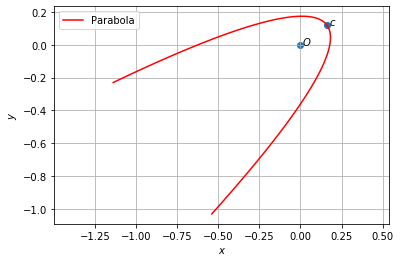
\includegraphics[width=\columnwidth]{./solutions/41/5/A6.png}
    \caption{Parabola with vertex c}
    \label{eq:solutions/41/5/fig:fig1}
\end{figure}
